\subsection{The protocol} \label{subsec:ecat-protocol}

The \emph{EtherCAT} protocol embeds its own frames into a standard \emph{Ethernet} frame, signing it with an hexadecimal value of $\mathtt{0x88A4}$ on the \emph{Ethernet}'s type header field.
Other protocol stacks like TCP/IP or UDP/IP can be used concurrently with \emph{EtherCAT}, but they are not required.
These are encapsulated into a separate mailbox so they do not disrupt real-time process data transmissions.
The fact that this network does not use these stacks means it has lower communication overhead.

The \emph{EtherCAT} frames are, themselves, divided into several datagrams, as show in \autoref{fig:ecat-frame}.
These can be addressed to specific devices using their node address or be sent to multiple devices, concurrently, using a logical address.
The datagram header contains information about the type of operation to perform, which can be one of three options: read, write of concurrent read-write operations.

\begin{figure}[htp]
	\centering
	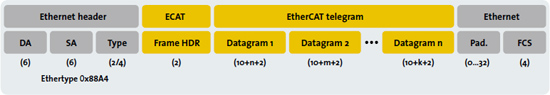
\includegraphics[width=1\textwidth]{EtherCAT_Technology_01_Protocol.jpg}
	\caption{EtherCAT frame structure \cite{protocol:ethercat}}
	\label{fig:ecat-frame}
\end{figure}

Datagrams include all information regarding data access which permit the master device to decide what data to access and when, meaning a fixed process data structure is not required.
Effectively, master devices can update variables with different cycle times, possibly relieving some processing power.
As an example, for a system that requires motion control, the motor drives can get their parameters updated with a 1ms period, while discrete Inputs/Outputs (I/Os) can be updated with a 20ms period (typical control applications).

Each slave contains a unique node address which is assigned during network configuration.
Because node addresses are static, they can be used to target the specific node, even if the underlying network topology changes.
In addition, slaves can also be addressed by their location on the network, but this is usually only used during network initialisation to check for topology changes.
This is done by comparing a configured list of node addresses and their location on the network with the discovered topology.

On system initialisation, multiple logical addresses can be configured on each node, allowing a single datagram to target multiple physical devices.
The cyclical exchange of process information uses logical addressing to execute the data transfers.

This type of addressing scheme also allows slave-to-slave communication.
There are two possibilities of achieving this:
\begin{enumerate}
	\item If the process structure is constant, sending data to another slave which is further downstream can be done in the same bus cycle;
	\item If the process is not constant or the network has a dynamic topology, slave-to-slave communication can go through the master device and, because of \emph{EtherCAT}'s performance, this is still faster than other traditional communication stacks (TCP/IP, UDP/IP, etc.).
\end{enumerate}

EtherCAT can also benefit from the modern system's \textbf Direct \textbf Memory \textbf Access (DMA) feature, which removes the necessity for a CPU to explicitly transfer data from physical RAM to a peripheral device.
This means that a master device application only needs to construct the EtherCAT frame and place it on a specific memory region, leaving the DMA controller to actually pass the data over to the Ethernet MAC controller, saving CPU for the actual data processing.
